\normalfalse \difficiletrue \tdifficilefalse
\correctionfalse

%\UPSTIidClasse{12} % 11 sup, 12 spé
%\newcommand{\UPSTIidClasse}{12}

\exer{Mouvement RR -- RSG  $\star\star$ \label{C2:08:46}}
\setcounter{question}{0}\UPSTIcompetence[2]{C2-08}
\UPSTIcompetence[2]{C2-09}
\index{Compétence C2-08}
\index{Compétence C2-09}
\index{Torseur cinétique}
\index{Torseur dynamique}
\index{Mécanisme à 2 rotations et RSG}
\ifcorrection
\else
\marginnote{\textbf{Pas de corrigé pour cet exercice.}}
\fi

\ifprof
\else
Soit le mécanisme suivant. On a $\vect{IA}=R\vect{j_0}$ et $\vect{AB}=L\vect{i_1}$. De plus $R=\SI{15}{mm}$.
On fait l'hypothèse de roulement sans glissement au point $I$. De plus :
\begin{itemize}
\item $G_1$ désigne le centre d'inertie de \textbf{1} tel que $\vect{AG_1}=-\ell\vect{i_1}$, on note $m_1$ la masse de \textbf{1} et $\inertie{G_1}{1}=\matinertie{A_1}{B_1}{C_1}{0}{0}{0}{\bas{1}}$; 
\item $G_2=B$ désigne le centre d'inertie de \textbf{2}, on note $m_2$ la masse de \textbf{2} et $\inertie{G_2}{2}=\matinertie{A_2}{B_2}{C_2}{0}{0}{0}{\bas{2}}$.
\end{itemize}
\begin{center}
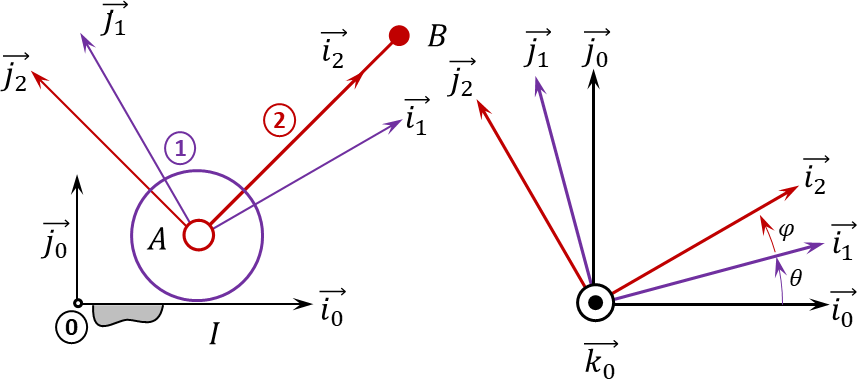
\includegraphics[width=\linewidth]{01}
\end{center}
\fi

\question{Déterminer $\vectrd{2}{0}\cdot \vect{i_1}$}
\ifprof
(Voir exercice B2-13 46-RR-RSG).
\begin{enumerate}
\item $\vectv{B}{2}{0} = L\varphip(t)\vj{2} +\thetap(t)\left(L\vj{1}-R\vi{0}\right) $.
\item  $\torseurcin{V}{2}{0} = \torseurl{\vecto{2}{0}=\left( \varphip(t)+\thetap(t) \right) \vk{0} }{ L\varphip(t)\vj{2} +\thetap(t)\left(L\vj{1}-R\vi{0}\right)}{B}$.
\item $\vectg{B}{2}{0} =  L\varphipp(t)\vj{2}-L\varphip(t)\left(\varphip(t)+\thetap(t) \right)\vi{2}  + \thetapp(t)\left(L\vj{1}-R\vi{0}\right) - L\thetap^2(t)\vi{1}$.
\end{enumerate} 

$\vectrd{2}{0}\cdot \vect{i_1} = m_2 \vectg{B}{2}{0} \cdot \vi{1}$
$ =\left( L\varphipp(t)\vj{2}-L\varphip(t)\left(\varphip(t)+\thetap(t) \right)\vi{2}  + \thetapp(t)\left(L\vj{1}-R\vi{0}\right) - L\thetap^2(t)\vi{1} \right) \cdot \vi{1}$
$ = -\sin\varphi(t) L\varphipp(t)-L\varphip(t)\left(\varphip(t)+\thetap(t) \right)\cos\varphi  + \thetapp(t)\left(L\vj{1}-R\vi{0}\right) - L\thetap^2(t)$


\else
\fi



\question{Déterminer $\vectmd{A}{2}{0}\cdot \vect{k_0}$}
\ifprof

Calculons $\vectmc{B}{2}{0} = \matinertie{A_2}{B_2}{C_2}{0}{0}{0}{\bas{2}} \vecto{2}{0} = C_2 \left(\varphip + \thetap \right) \vk{0}$.

Calculons $\vectmd{B}{2}{0} = C_2 \left(\varphipp + \thetapp\right) \vk{0}$.

Enfin, $ \babardp{A}{B}{2}{0}{\vk{0}}$  

$=C_2 \left(\varphipp + \thetapp\right)  + m_2 \left( L\vect{i_1} \wedge \left( L\varphipp(t)\vj{2}-L\varphip(t)\left(\varphip(t)+\thetap(t) \right)\vi{2}  + \thetapp(t)\left(L\vj{1}-R\vi{0}\right) - L\thetap^2(t)\vi{1} \right)\right) \cdot \vk{0}$

$=C_2 \left(\varphipp + \thetapp\right)  + m_2 L \left( \left( L\varphipp(t)\vect{i_1} \wedge\vj{2}-L\varphip(t)\left(\varphip(t)+\thetap(t) \right)\vect{i_1} \wedge\vi{2}  + \thetapp(t)\left(L\vect{i_1} \wedge\vj{1}-R\vect{i_1} \wedge\vi{0}\right)  \right)\right) \cdot \vk{0}$


$=C_2 \left(\varphipp + \thetapp\right)  + m_2 L  \left( L\varphipp(t)\cos\varphi-L\varphip(t)\left(\varphip(t)+\thetap(t) \right)\sin\varphi  + \thetapp(t)\left(L+R\sin \theta\right)  \right) $.

\else
\fi

\question{Déterminer $\vectmd{I}{1+2}{0}\cdot \vect{k_0}$}
\ifprof

Calculons 
$R\vect{j_0} \wedge \left(L\varphipp(t)\vj{2}-L\varphip(t)\left(\varphip(t)+\thetap(t) \right)\vi{2}  + \thetapp(t)\left(L\vj{1}-R\vi{0}\right) - L\thetap^2(t)\vi{1}\right) \cdot \vect{k_0} $ 

$= R \left(L\varphipp(t)\vect{j_0} \wedge \vj{2}-L\varphip(t)\left(\varphip(t)+\thetap(t) \right)\vect{j_0} \wedge \vi{2}  + \thetapp(t)\left(L\vect{j_0} \wedge \vj{1}-R\vect{j_0} \wedge \vi{0}\right) - L\thetap^2(t)\vect{j_0} \wedge \vi{1}\right) \cdot \vect{k_0} $


$= R \left(L\varphipp(t)\sin\left(\theta+\varphi\right)+L\varphip(t)\left(\varphip(t)+\thetap(t) \right)\cos\left( \varphi + \theta\right)   + \thetapp(t)\left(L\sin\theta+R\right) + L\thetap^2(t)\cos \theta\right)  $...

On peut en déduire $\vectmd{I}{2}{0}\cdot \vect{k_0}$.


\textbf{On fait l'hypothèse que $\ell = 0$}.


Par ailleurs, on a $\vectmd{G_1}{1}{0} = C_1 \thetapp (t) \vk{0}$

>> Calculer $\vectmd{I}{1}{0}$...

\else
\fi


\ifprof
\else
\begin{flushright}
\footnotesize{Corrigé  voir \ref{C2:08:46}.}
\end{flushright}%
\fi